
\section{Основные определения}

Ниже приведен список терминов, с которым необходимо ознакомиться перед ознакомлением с работой [1.1] 

\textbf{Биржа (Market, Exchange)} - финансовый инструмент, обеспечивающий проведение сделок по купли-продаже предметов торговли (товары, акции, сырье и т.п.).

\textbf{Торговая заявка (Order)} - заявка на покупку или продажу определенного объема (volume) по определенной цене (price).


\textbf{Направление заявки (Direction)} - действие, которое заявка хочет совершить. Это может быть продажа (BID) или покупка (ASK).

\textbf{Котировка (Quote)} - объединение заявок с одной ценой и одним направлением.

\textbf{Сделка (Trade)} - заключение договора по фиксированной цене между двумя заявками противоположных направлений.

\textbf{Пассивная торговая заявка (Passive Order)} - заявка, которая при поступлении на биржу не приводит к немедленным сделкам.

\textbf{Активная торговая заявка (Active Order)} - заявка, которая при поступлении на биржу приводит к немедленным сделкам.

\textbf{Биржевой стакан (Order Book)} - механизм распределения заявок на покупку и продажу, обеспечивающий их упорядоченность в порядке уменьшения ценовой выгоды внутри одного направления.

\textbf{Торговый движок (Matching Engine)} - сущность, реализуюзая всю механику по постановке заявок в биржевой стакан и проведению сделок.

\textbf{Маркет мейкер (Market maker)} - участник торгов, отправляющий только пассивные заявки.

\textbf{Волатильность (Volatility)} - характеристика скорости изменчивости цены во время торгов. В этой работе под этим также будет подразумеваться характеристика объема присылаемых клиентами заявок.

\newpage

\section{Введение}

Одной из самых сложных и интересных с точки зрения реализации задач в финансах
является реализация внутренней инфрастурктуры биржи: это должна быть отказоустойчивая, высокопроизводительная и легко расширяемая в производственных мощностях архитектура.

Современные биржи состоят из большого количества асинхронных компонент, каждая из которых может потреблять различное количество ресурсов, в зависимости от объема заявок от участников торгов, которые необходимо обработать в моменте.

В первой части этой работы будет реализованная биржа, имеющая стандартную архитектуру со всеми основными компонентами, используемыми в реальных торгах. Мы обсудим технические аспекты, а также проведем нагрузочное тестирование, чтобы выяснить какой объем заявок написанная биржа сможет обработать.

Затем будут рассмотрены и применены механизмы предсказания волатильности, обеспечивающие повышенную отказоустойчивость биржи. 

  
\section{Как работает биржа}

Прежде, чем перейти к реализации, необходимо привести алгоритм сведения заявок, по которому работают биржи. Этот фундаментальный принцип лежит в основе всех торгов во всем мире.

Все устроено довольно просто. Как мы уже знаем, всегда существует некоторый предмет торговли, который кто-то хочет продать, а кто-то хочет купить. Далее встает вопрос: как организовать торги таким образом, чтобы было честное и эффективное распределение сделок?
\newpage

Для этого существует механизм \textbf{биржевого стакана}. Он работает следующим образом: \textbf{заявки на покупку} сортируются в порядке уменьшения цены, а \textbf{заявки на продажу} - в порядке увеличения. Далее \textbf{внутри каждой цены} создается очередь заявок, в порядке их прихода на биржу. Такая очередь и называется \textbf{котировкой}. Таким образом, образуются два \textbf{направления торговли}, состоящие из котировок.


\begin{center}
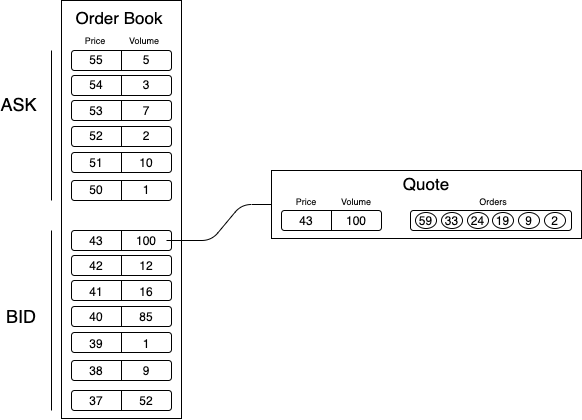
\includegraphics[width=450pt]{images/order_book_schema.png}
\end{center}

\newpage

В какой-то момент приходит заявка на покупку (продажу), которая по цене пересекает противоположное направление продажи (покупки). То есть находятся такие уже стоящие в стакане другие заявки на продажу (покупку), цена которых больше (меньше), и с ними можно организовать сделку. Заявка на покупку (продажу), спровоцировавшая такую сделку называется \textbf{активной}, а заявка на продажу (покупку), уже стоящая в стакане, называется \textbf{пассивной}. Выполнение этой логики обеспечивается \textbf{торговым движком}.


\begin{center}
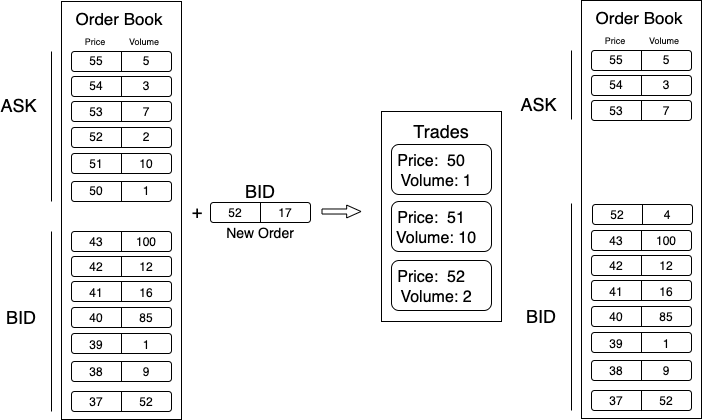
\includegraphics[width=450pt]{images/trade_schema.png}
\end{center}

Таким образом, участники торгов наглядно видят, сколько объема и по какой цене они могут купить или продать прямо сейчас активной заявкой, либо на какую цену они могут отправить пассивную заявку, чтобы ждать сделки в будущем.

\pagebreak
